\documentclass[aspectratio=169, 9pt]{beamer}

% Packages for math and formatting
\usepackage{amsmath}
\usepackage{booktabs}
\usepackage{graphicx}

% Custom Technical Color Scheme
\definecolor{TechBlue}{RGB}{20, 75, 150}
\definecolor{TechGrey}{RGB}{245, 245, 245}
\definecolor{AccentOrange}{RGB}{200, 80, 0}

\setbeamercolor{palette primary}{bg=TechBlue,fg=white}
\setbeamercolor{structure}{fg=TechBlue}
\setbeamercolor{frametitle}{bg=TechGrey, fg=TechBlue}
\setbeamercolor{item}{fg=AccentOrange}

% Space-saving formatting
\setbeamertemplate{navigation symbols}{} % Removes bottom navigation bar
\setbeamertemplate{footline}[frame number] % Minimalist slide numbering
\setbeamersize{text margin left=6mm, text margin right=6mm} % Widens the usable area
\setlength{\leftmargini}{0.5cm} % Tighter bullet point indentation

\title{State Estimation for Quadruped Robots on Non-Stationary Terrain}
\subtitle{via Invariant Extended Kalman Filter and Disturbance Observer}
\author{Esraaj Sarkar Gupta, Kanishk Khandelwal, Manan Gadesha}
\date{\today}

\begin{document}

% --- TITLE SLIDE ---
\begin{frame}
    \titlepage
\end{frame}

% --- SLIDE 1 ---
\begin{frame}[t]{1. The Bottleneck in Quadruped State Estimation}
    \textbf{The Context \& Challenge}
    % SPEAKER NOTES: With the increasing use of quadruped robots in more demanding scenarios, ensuring accurate and stable state estimation in complex environments has become particularly important. State estimation suffers in non-stationary terrain from (as listed) foot-end slippage, or unstable contact. This leads to significant state drift in state estistions multi-sensor fusion models.
    
    \begin{itemize}
        \item As quadrupeds are deployed in more demanding environments, the importance of precise state estimation grows.
        \item Existing state estimation algorithms often face challenges on non-stationary terrains due to issues like foot-end slippage or unstable contact, leading to significant state drift.
    \end{itemize}

    \vspace{0.5cm}
    
    \textbf{Slippage introduces non-Gaussian errors that compound over time and cause unbounded drift.}

    \vspace{0.5cm}
    \textbf{This paper solves this problem by introducing an extended Kalman Filter}
    \begin{itemize}
        \item The foot-end slippage is modeled through a deviation of body velocity.
        \item This work then utilizes the velocity deviation estimation to reduce the drift caused by foot-end slippage.
        \item The estimator is applied by engineering a right-invariant extended Kalman filter (RI EKF), by fusing foot-end velocity and position observations (measurements).
    \end{itemize}
    

\end{frame}

% --- SLIDE 2 ---
\begin{frame}[t]{2. InEKF \& Velocity Bias}
    % The SE_7(3) State Matrix -- Special Euclidean Group in 7D
    \begin{equation}
        X_t = 
        \begin{bmatrix} 
        R_{WB}(t) & {}_Wv_B(t) & {}_Wp_B(t) & {}_Wp_{f_1}(t) & {}_Wp_{f_2}(t) & {}_Wp_{f_3}(t) & {}_Wp_{f_4}(t) & b_B^v(t) \\ 
        0_{7,3} & \multicolumn{7}{c}{I_7} 
        \end{bmatrix}
    \end{equation}

    % SPEAKER NOTES: The state estimator is capable of estimating for all the values here.
    {\tiny
    \textbf{State Variables Breakdown:}
    \begin{itemize}
        \item $R_{WB}(t)$: Robot body's orientation (Rotation matrix).
        \item ${}_Wv_B(t), \ {}_Wp_B(t)$: Robot body's velocity and position in the world frame.
        \item ${}_Wp_{f_i}(t)$: Positions of the four feet.
        \item $b_B^v(t)$: The velocity bias term capturing the slip.
    \end{itemize}
    }

    The state evolves deterministically using a differential equation driven by IMU inputs.

    \begin{equation}
        \frac{d}{dt}\hat{X}_t = f_{u_t}\big(\hat{X}_t\big)
    \end{equation}

    % The Riccati Equation (and whatnot)
    The error (covariance) is propagated with the Riccati Equation

    \begin{equation}
        \frac{d}{dt}P_{t} = A_{t}P_{t} + P_{t}A_{t}^{T} + \overline{Q}_{t}
    \end{equation}
    \vspace{0.2cm}

    {\tiny
        \textbf{Term Breakdown:}
        \begin{itemize}
            \item $P_{t}$: The current state covariance matrix.
            \item $A_{t}$: The linearized system dynamics matrix. It dictates how the robot's physical movement stretches the existing uncertainty.
            \item $\overline{Q}_{t}$: The process noise covariance, representing the continuous injection of raw sensor noise.
                \item Calculated as $\overline{Q}_{t} = Ad_{\hat{X}}Cov(n_{t})Ad_{\hat{X}}$.
        \end{itemize}
    }
\end{frame}

% --- SLIDE 3 ---
\begin{frame}[t]{3. Measurement Model \& Contact Probability}
    \textbf{Dual Proprioceptive Observations}
    \begin{itemize}
        \item To correct the predicted state, the filter fuses both foot-end position (via forward kinematics) and velocity (via leg Jacobian) into a single observation model.
        % SPEAKER NOTES: This results in an over-constrained system. 
    \end{itemize}

    \vspace{0.3cm}
    \textbf{Handling Unstable Contact}
    % SPEAKER NOTES: The robot uses joint torques to calculate the ground reaction force (GRF). It feeds this into a logistic regression model to find the probability that the foot is actually planted.
    \begin{itemize}
        \item On non-stationary terrain, foot contact is unreliable. The filter computes a stable contact probability based on the z-axis ground reaction force ($f_{z,i}^{k}$):
    \end{itemize}
    
    \begin{equation}
        P_{k}(S_{i}=1|f_{k}^{i}) = \frac{1}{1+exp(-\beta_{1}f_{z,i}^{k}-\beta_{2})}
    \end{equation}
    % This is a logistic distribution with hyperparameters beta1 and beta2

    \vspace{0.3cm}
    \textbf{Adaptive Covariance \& The InEKF Update}
    \begin{itemize}
        \item If contact probability drops, the noise covariance ($\Sigma_{t}^{p_{f_{i}}}$) is dynamically inflated, mitigating the impact of slipping data:
    \end{itemize}
    
    \begin{equation}
        \Sigma_{t}^{p_{f_{i}}}(k) = \big(1+L(1-P_{k}(S_{i}=1|f_{k}^{i}))\big)\Sigma_{t}^{p_{f_{i}}}(k)
    \end{equation}

    % SPEAKER NOTES: Finally, the state matrix is updated using the Exponential map to ensure the correction stays perfectly wrapped on the curved SE_7(3) Lie group manifold.
    {\tiny
    \textbf{Right-Invariant Update Step:}
    \begin{itemize}
        \item The state is updated using the Exponential map of the Lie group: $X_{t}^{+} = Exp(K_{t}z_{t})\hat{X}_{t}$
        \item The covariance is shrunk to reflect new certainty: $P_{t}^{+} = (I-K_{t}C_{t})P_{t}$
    \end{itemize}
    }
\end{frame}

% --- SLIDE 4 ---
\begin{frame}[t]{4. Experimental Results \& Analysis}
    \begin{columns}[T]
        % Left Column: Text and Data
        \begin{column}{0.55\textwidth}
            \textbf{Experimental Setup}
            \begin{itemize}
                \item \textbf{Hardware:} Jueying Mini quadruped robot equipped with an IMU and 12 joint encoders (operating at 166 Hz).
                \item \textbf{Ground Truth:} Outdoor testing required using LiDAR SLAM (LIO-SAM) as the trajectory baseline.
                \item \textbf{Environments:} Tested across three non-stationary terrains: Rugged slopes, shallow grass, and deep grass.
            \end{itemize}

            \vspace{0.2cm}
            \textbf{Trajectory Evaluation (ATE RMSE)}
            \begin{table}[]
                \centering
                \resizebox{\textwidth}{!}{
                \renewcommand{\arraystretch}{1.2}
                \begin{tabular}{lccc}
                    \toprule
                    \textbf{Terrain} & \textbf{QEKF} & \textbf{InEKF (Vel)} & \textbf{Proposed} \\
                    \midrule
                    Rugged Slopes & 1.345 m & 1.589 m & \textbf{0.457 m} \\
                    Shallow Grass & 0.789 m & 2.374 m & \textbf{0.343 m} \\
                    Deep Grass & 0.599 m & 3.381 m & \textbf{0.528 m} \\
                    \bottomrule
                \end{tabular}
                }
            \end{table}
        \end{column}
        
        % Right Column: Image Placeholder
        \begin{column}{0.4\textwidth}
            \centering
            \vspace{0.5cm}
            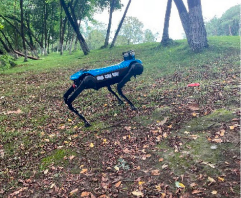
\includegraphics[width=\textwidth]{rugged_slopes.png}
            \begin{center}
                \textit{Quadruped on rugged slopes}
            \end{center}
        \end{column}
    \end{columns}
\end{frame}

% --- SLIDE 5 ---
\begin{frame}[t]{5. Conclusions \& Future Trajectory}
    \begin{columns}[T]
        % Left Column: Text
        \begin{column}{0.55\textwidth}
            \textbf{Core Contributions}
            \begin{itemize}
                \item \textbf{Slip as a State:} Explicitly modeling foot-end slippage as a velocity deviation term drastically reduces unbounded position drift on non-stationary terrains.
                \item \textbf{Robust Proprioception:} Fusing dual kinematic observations (position and velocity) with a GRF-based contact probability model creates a highly robust state estimator.
            \end{itemize}

            \vspace{0.4cm}
            \textbf{Future Research Directions}
            \begin{itemize}
                \item \textbf{Exteroceptive Fusion:} Integrating external perception sensors (vision cameras, LiDAR) to further enhance localization and mapping.
                \item \textbf{Extreme Terrains:} Adapting the filter to handle rapidly changing surface properties or dynamic obstacles.
                \item \textbf{Computational Efficiency:} Optimizing the matrix operations to achieve lower-latency real-time state estimation.
            \end{itemize}
        \end{column}

        % Right Column: Image Placeholder
        \begin{column}{0.4\textwidth}
            \centering
            \vspace{1cm}
            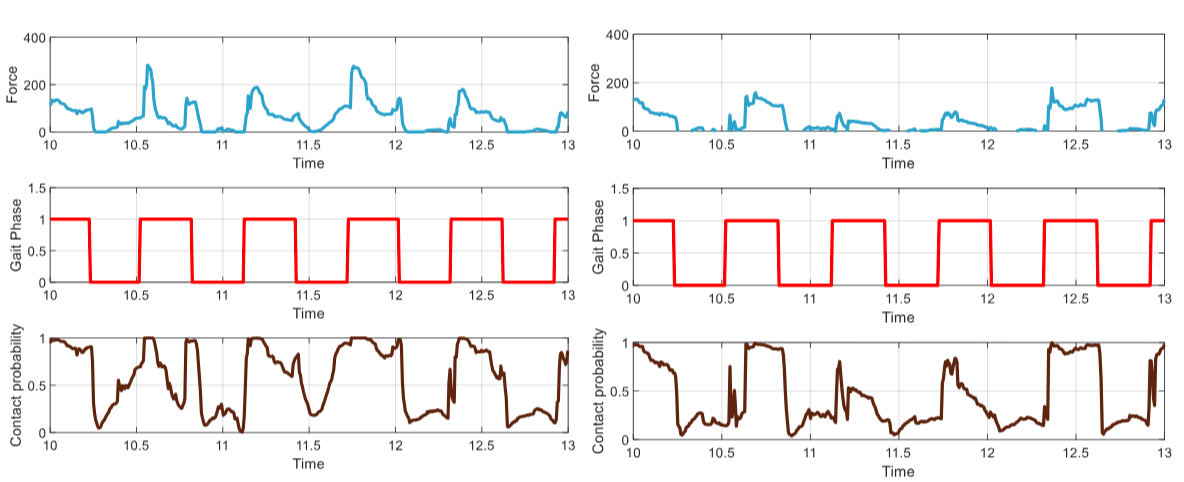
\includegraphics[width=\textwidth]{contact_probabilities.png}
            \begin{center}
                \textit{Contact Probability Graph, Right and Left legs}
            \end{center}
        \end{column}
    \end{columns}
\end{frame}

\end{document}